\documentclass{wissdoc}

% Autor: Roland Bless 1996-2009, bless <at> kit.edu
% ----------------------------------------------------------------
% Diplomarbeit - Hauptdokument
% ----------------------------------------------------------------
%%
%% $Id: diplarb.tex 53 2009-12-10 12:23:37Z bless $
%%
% wissdoc Optionen: draft, relaxed, pdf --> siehe wissdoc.cls
% ------------------------------------------------------------------
% Weitere packages: (Dokumentation dazu durch "latex <package>.dtx")
%\usepackage{bibgerm}
%\usepackage[backend=biber]{biblatex} 
\usepackage{csquotes} 
\usepackage{tabularx}
\usepackage{booktabs}
\usepackage{multirow}
%\usepackage{tocbibind}
\usepackage{siunitx}
\usepackage{xcolor}
\usepackage{textcomp}
\usepackage{listings}
\usepackage{newfloat,caption}
\usepackage{subcaption}
\usepackage{footnote}
\usepackage{rotating}
\usepackage{pgfplots}
\usepackage{pgfplotstable}
\usepackage{url}
\usepackage{boxhandler}
\usepackage{tabu}
\usepackage{amssymb}
%\usepackage{subfig}
%\usepackage{subcaption}
\usepackage{caption}
\usepackage{subcaption}
%\usepackage[plainpages=true]{hyperref}
\usepackage[space]{grffile}
%\usepackage[numbers,sort&compress]{natbib}
\usepackage[backend=bibtex8,natbib=true,hyperref=true,doi=false,url=false,sorting=none]{biblatex}
% \usepackage{varioref}
% \usepackage{verbatim}
\usepackage{float}    %z.B. \floatstyle{ruled}\restylefloat{figure}
%\usepackage[hidelinks]{hyperref}
% \usepackage{subfigure}
% \usepackage{fancybox} % für schattierte,ovale Boxen etc.
% \usepackage{tabularx} % automatische Spaltenbreite
% \usepackage{supertab} % mehrseitige Tabellen
% \usepackage[svnon,svnfoot]{svnver} % SVN Versionsinformation 
%% ---------------- end of usepackages -------------

%\svnversion{$Id: diplarb.tex 53 2009-12-10 12:23:37Z bless $} % In case that you want to include version information in the footer
%\hyphenation{if...-then...}
%% Informationen für die PDF-Datei
\pgfplotsset{compat=newest}

\hypersetup{
%%% styling of link inside pdf
  colorlinks,
  citecolor=black,
  filecolor=black,
  linkcolor=black,
  urlcolor=black,
%%%		
 pdfauthor={FirstName LastName},
 pdftitle={Title of Thesis}
 pdfsubject={Not set},
 pdfkeywords={Not set}
}
\DeclareFloatingEnvironment[fileext=frm,placement={!ht},name=Listing,within=section]{listing}

% Macros, nicht unbedingt notwendig
%%%%%%%%%%%%%%%%%%%%%%%%%%%%%%%%%%%%%%%%%%%%%%%%%%%%%%%%%%
% macros.tex -- einige mehr oder weniger nuetzliche Makros
% Autor: Roland Bless 1998
%%%%%%%%%%%%%%%%%%%%%%%%%%%%%%%%%%%%%%%%%%%%%%%%%%%%%%%%%%
% $Id: macros.tex 33 2007-01-23 09:00:59Z bless $
%%%%%%%%%%%%%%%%%%%%%%%%%%%%%%%%%%%%%%%%%%%%%%%%%%%%%%%%%%


%%%%%%%%%%%%%%%%%%%%%%%
% Kommentare 
%%%%%%%%%%%%%%%%%%%%%%%
\ifnotdraftelse{
\newcommand{\Kommentar}[1]{}
}{\newcommand{\Kommentar}[1]{{\em #1}}}
% Alles innerhalb von \Hide{} oder \ignore{} 
% wird von LaTeX komplett ignoriert (wie ein Kommentar)
\newcommand{\Hide}[1]{}
\let\ignore\Hide

%%%%%%%%%%%%%%%%%%%%%%%%%
% Leere Seite ohne Seitennummer, wird aber gezaehlt
%%%%%%%%%%%%%%%%%%%%%%%%%

\newcommand{\leereseite}{% Leerseite ohne Seitennummer, n�chste Seite rechts (wenn 2-seitig)
 \clearpage{\pagestyle{empty}\cleardoublepage}
}
%%%%%%%%%%%%%%%%%%%%%%%%%%
% Flattersatz rechts und Silbentrennung, Leerraum nach rechts maximal 1cm
%%%%%%%%%%%%%%%%%%%%%%%%%%
\makeatletter
\newcommand{\myraggedright}{%
 \let\\\@centercr\@rightskip 0pt plus 1cm
 \rightskip\@rightskip
  \leftskip\z@skip
  \parindent\z@
  \spaceskip=.3333em
  \xspaceskip=.5em}
\makeatother

\makeatletter
\newcommand{\mynewline}{%
 \@centercr\@rightskip 0pt plus 1cm
}
\makeatother


%%%%%%%%%%%%%%%%%%%%%%%%%%
% F�r Index
%%%%%%%%%%%%%%%%%%%%%%%%%%
\makeatletter
\def\mydotfill{\leavevmode\xleaders\hb@xt@ .44em{\hss.\hss}\hfill\kern\z@}
\makeatother
\def\bold#1{{\bfseries #1}}
\newbox\dbox \setbox\dbox=\hbox to .4em{\hss.\hss} % dot box for leaders
\newskip\rrskipb \rrskipb=.5em plus3em % ragged right space before break
\newskip\rrskipa \rrskipa=-.17em plus -3em minus.11em % ditto, after
\newskip\rlskipa \rlskipa=0pt plus3em % ragged left space after break
\newskip\rlskipb \rlskipb=.33em plus-3em minus.11em % ragged left before break
\newskip\lskip \lskip=3.3\wd\dbox plus1fil minus.3\wd\dbox % for leaders
\newskip \lskipa \lskipa=-2.67em plus -3em minus.11em %after leaders
\mathchardef\rlpen=1000 \mathchardef\leadpen=600
\def\rrspace{\nobreak\hskip\rrskipb\penalty0\hskip\rrskipa}
\def\rlspace{\penalty\rlpen\hskip\rlskipb\vadjust{}\nobreak\hskip\rlskipa}
\let\indexbreak\rlspace
\def\raggedurl{\penalty10000 \hskip.5em plus15em \penalty0 \hskip-.17em plus-15em minus.11em}
\def\raggeditems{\nobreak\hskip\rrskipb \penalty\leadpen \hskip\rrskipa %
\vadjust{}\nobreak\leaders\copy\dbox\hskip\lskip %
\kern3em \penalty\leadpen \hskip\lskipa %
\vadjust{}\nobreak\hskip\rlskipa}
\renewcommand*\see[2]{\rlspace\emph{\seename}~#1} % from makeidx.sty

%%%%%%%%%%%%%%%%%%%%%%%%%%
% Neue Seite rechts, leere linke Seite ohne Headings
%%%%%%%%%%%%%%%%%%%%%%%%%%
\newcommand{\xcleardoublepage}
{{\pagestyle{empty}\cleardoublepage}}

%%%%%%%%%%%%%%%%%%%%%%%%%%
% Tabellenspaltentypen (benoetigt colortbl)
%%%%%%%%%%%%%%%%%%%%%%%%%%
\newcommand{\PBS}[1]{\let\temp=\\#1\let\\=\temp}
\newcolumntype{y}{>{\PBS{\raggedright\hspace{0pt}}}p{1.35cm}}
\newcolumntype{z}{>{\PBS{\raggedright\hspace{0pt}}}p{2.5cm}}
\newcolumntype{q}{>{\PBS{\raggedright\hspace{0pt}}}p{6.5cm}}
\newcolumntype{g}{>{\columncolor[gray]{0.8}}c} % Grau
\newcolumntype{G}{>{\columncolor[gray]{0.9}}c} % helleres Grau

%%%%%%%%%%%%%%%%%%%%%%%%%%
% Anf�hrungszeichen oben und unten
%%%%%%%%%%%%%%%%%%%%%%%%%%
\newcommand{\anf}[1]{"`{#1}"'}

%%%%%%%%%%%%%%%%%%%%%%%%%%
% Tiefstellen von Text
%%%%%%%%%%%%%%%%%%%%%%%%%%
% S\tl{0} setzt die 0 unter das S (ohne Mathemodus!)
% zum Hochstellen gibt es uebrigens \textsuperscript
\makeatletter
\DeclareRobustCommand*\textlowerscript[1]{%
  \@textlowerscript{\selectfont#1}}
\def\@textlowerscript#1{%
  {\m@th\ensuremath{_{\mbox{\fontsize\sf@size\z@#1}}}}}
\let\tl\textlowerscript
\let\ts\textsuperscript
\makeatother

%%%%%%%%%%%%%%%%%%%%%%%%%%
% Gau�-Klammern
%%%%%%%%%%%%%%%%%%%%%%%%%%
\newcommand{\ceil}[1]{\lceil{#1}\rceil}
\newcommand{\floor}[1]{\lfloor{#1}\rfloor}

%%%%%%%%%%%%%%%%%%%%%%%%%%
% Average Operator (analog zu min, max)
%%%%%%%%%%%%%%%%%%%%%%%%%%
\def\avg{\mathop{\mathgroup\symoperators avg}}

%%%%%%%%%%%%%%%%%%%%%%%%%%
% Wortabk�rzungen
%%%%%%%%%%%%%%%%%%%%%%%%%%
\def\zB{z.\,B.\ }
\def\dh{d.\,h.\ }
\def\ua{u.\,a.\ }
\def\su{s.\,u.\ }
\newcommand{\bzw}{bzw.\ }

%%%%%%%%%%%%%%%%%%%%%%%%%%%%%%%%%%%
% Einbinden von Graphiken
%%%%%%%%%%%%%%%%%%%%%%%%%%%%%%%%%%%
% global scaling factor
\def\gsf{0.9}
%% Graphik, 
%% 3 Argumente: Datei, Label, Unterschrift
\newcommand{\Abbildung}[3]{%
\begin{figure}[tbh] %
\centerline{\scalebox{\gsf}{\includegraphics*{#1}}} %
\caption{#3} %
\label{#2} %
\end{figure} %
}
\let\Abb\Abbildung
%% Abbps
%% Graphik, skaliert, Angabe der Position
%% 5 Argumente: Position, Breite (0 bis 1.0), Datei, Label, Unterschrift
\newcommand{\Abbildungps}[5]{%
\begin{figure}[#1]%
\begin{center}
\scalebox{\gsf}{\includegraphics*[width=#2\textwidth]{#3}}%
\caption{#5}%
\label{#4}%
\end{center}
\end{figure}%
}
\let\Abbps\Abbildungps
%% Graphik, Angabe der Position, frei w�hlbares Argument f�r includegraphics
%% 5 Argumente: Position, Optionen, Datei, Label, Unterschrift
\newcommand{\Abbildungpf}[5]{%
\begin{figure}[#1]%
\begin{center}
\scalebox{\gsf}{\includegraphics*[#2]{#3}}%
\caption{#5}%
\label{#4}%
\end{center}
\end{figure}%
}
\let\Abbpf\Abbildungpf

%%
% Anmerkung: \resizebox{x}{y}{box} skaliert die box auf Breite x und H�he y,
%            ist x oder y ein !, dann wird das uspr�ngliche 
%            Seitenverh�ltnis beibehalten.
%            \rescalebox funktioniert �hnlich, nur das dort ein Faktor
%            statt einer Dimension angegeben wird.
%%
% \Abbps{Position}{Breite in Bruchteilen der Textbreite}{Dateiname}{Label}{Bildunterschrift}
%

\newcommand{\refAbb}[1]{%
s.~Abbildung \ref{#1}}

%%%%%%%%%%%%%%%%%%%%
%% end of macros.tex
%%%%%%%%%%%%%%%%%%%%

% Print URLs not in Typewriter Font
\def\UrlFont{\rm}

\newcommand{\specialcell}[2][c]{%
  \begin{tabular}[#1]{@{}c@{}}#2\end{tabular}}

\newcommand\todo[1]{\textcolor{red}{TODO: #1}}

\newcommand\hlcode[1]{\textcolor{red}{#1}}

\newcommand\citeable[1]{\textcolor{green}{\hl{citeable: #1}}}

\newcolumntype{$}{>{\global\let\currentrowstyle\relax}}
\newcolumntype{^}{>{\currentrowstyle}}
\newcommand{\rowstyle}[1]{\gdef\currentrowstyle{#1}%
  #1\ignorespaces
}

\newif\ifcomment
%\commenttrue %# Show comments


%\newcommand{\blankpage}{% Leerseite ohne Seitennummer, nächste Seite rechts
% \clearpage{\pagestyle{empty}\cleardoublepage}
%}

\renewcommand{\thesection}{\arabic{section}}
%% Einstellungen für das gesamte Dokument

% Trennhilfen
% Wichtig! 
% Im german-paket sind zusätzlich folgende Trennhinweise enthalten:
% "- = zusätzliche Trennstelle
% "| = Vermeidung von Ligaturen und mögliche Trennung (bsp: Schaf"|fell)
% "~ = Bindestrich an dem keine Trennung erlaubt ist (bsp: bergauf und "~ab)
% "= = Bindestrich bei dem Worte vor und dahinter getrennt werden dürfen
% "" = Trennstelle ohne Erzeugung eines Trennstrichs (bsp: und/""oder)

% Trennhinweise fuer Woerter hier beschreiben
\hyphenation{
% Pro-to-koll-in-stan-zen
% Ma-na-ge-ment  Netz-werk-ele-men-ten
% Netz-werk Netz-werk-re-ser-vie-rung
% Netz-werk-adap-ter Fein-ju-stier-ung
% Da-ten-strom-spe-zi-fi-ka-tion Pa-ket-rumpf
% Kon-troll-in-stanz
}
\lstset{
    frame=single,
    breaklines=true,
		basicstyle=\scriptsize,
    %postbreak=\raisebox{0ex}[0ex][0ex]{\ensuremath{\color{red}\hookrightarrow\space}}
}

% Index-Datei öffnen
\ifnotdraft{\makeindex}
%%%%%%%%%%%%%% includeonly %%%%%%%%%%%%%%%%%%%
% Es werden nur die Teile eingebunden, die hier 
% aufgefuehrt sind!
\includeonly{%
titlepage,%
problemstellung,% Motivation, Zielsetzung, Gliederung
zielsetzung,% Grundlagen 
forschungsstand,   % Problembeschreibung (Detail) und Related Work
konzept,   % Beschreibung der Problemlösung (Konzepte, allg. Architektur, ...)
gliederung,  % Beschreibung der Umsetzung/Implementierung
zeitplan,      % Nachweis und Auswertung
}
\bibliography{Literature, Websites}
\usepgfplotslibrary{groupplots}
\usetikzlibrary{pgfplots.groupplots}
%\addbibresource{diplarb.bib}

%%%%%%%%%%%%%%%%%%%%%%%%%%%%%%%%%%%%%%%%%%%%%%
\begin{document}

%\frontmatter
\ifnotdraft{
 %% Titelseite
%% Vorlage $Id: titelseite.tex 54 2009-12-10 12:23:58Z bless $

\def\usesf{}
\let\usesf\sffamily % diese Zeile auskommentieren für normalen TeX Font

\newsavebox{\Erstgutachter}
\savebox{\Erstgutachter}{\usesf Prof.~Dr.~Michael Beigl}
\newsavebox{\Zweitgutachter}
\savebox{\Zweitgutachter}{\usesf Derzeit noch offen}

\begin{titlepage}
\setlength{\unitlength}{1pt}

\begin{picture}(0,0)(85,770)

\includegraphics[width=\paperwidth]{logos/KIT_Deckblatt}
\end{picture}

\vspace*{-39pt}\hspace*{300pt}
\includegraphics[width=.27\paperwidth]{logos/TECO_KIT}

\thispagestyle{empty}

%\begin{titlepage}
%%\let\footnotesize\small \let\footnoterule\relax
\begin{center}
\hbox{}
\vfill
{\usesf
{\huge\bfseries Konzeption und Entwicklung einer intuitiven Modellierungssprache für digitale Therapien mittels Chatbots
 \par}
\vskip 1.8cm
Expos\'{e} zur Masterarbeit\\
von\\[2mm]
\vskip 1cm

{\large\bfseries Luisa Andre\\}
Studiengang Informatik (M.Sc)\\
E-Mail: luisa.andre@student.kit.edu
\vskip 1.2cm
Lehrstuhl für Pervasive Computing Systeme/TECO\\
Institut für Telematik\\
Fakultät für Informatik\\
%Universität Karlsruhe (TH)\\[2ex]
\vskip 3cm
\begin{tabular}{p{5.5cm}l}
Erstgutachter: & \usebox{\Erstgutachter} \\
Zweitgutachter: & \usebox{\Zweitgutachter} \\
Betreuerin: & PD Dr. Andrea Schankin \\
\end{tabular}
\vskip 3cm
Projektzeitraum:\qquad 01.01.2019 -- 30.06.2019
}
\end{center}
\vfill
\end{titlepage}
%% Titelseite Ende


%%% Local Variables: 
%%% mode: latex
%%% TeX-master: "diplarb"
%%% End: 

}

%% ++++++++++++++++++++++++++++++++++++++++++
%% Hauptteil
%% ++++++++++++++++++++++++++++++++++++++++++
\graphicspath{{images/}}

%\mainmatter
%\null
\pagenumbering{arabic}
%% Einleitung.tex
%% $Id: einleitung.tex 28 2007-01-18 16:31:32Z bless $
%%

\section{Problemstellung}
\label{ch:Problemstellung}
%% ==============================
% CLEARLY SHOW CONTRIBUTIONS AND LINK THEM TO SECTIONS

%- Mit welchem Bereich beschäftigen wir uns?
%- Welche Probleme treten hier auf?
%- Wie werden diese bisher gelöst?
%- Was wollen wir beitragen?

Ob Depressionen, Burnout oder Angststörungen - psychische und Lebensstil assoziierte Erkrankungen wurden in den letzten Jahrzehnten immer wichtiger für die Gesellschaft. Seit 1998 weißt Deutschland einen Anstieg von Krankheitstagen, bedingt durch psychische Diagnosen, auf. Gleichzeitig wird ein Rückgang von Krankmeldungen durch andere Diagnosen registriert. (vgl. \cite{Jacobi2014}, S. 85) Durch diese Entwicklung stieg der Bedarf an psychotherapeutischen Behandlungsplätzen, welcher sich an den Wartezeiten für eine psychotherapeutische Behandlung bemerkbar macht. Derzeit liegen diese im Schnitt bei 5,7 Wochen (vgl. \cite{Microsof77:online}, S.5). Auch Krankenkassen beobachten den Anstieg der psychischen Diagnosen. So betont Prof. Dr. Christoph Straub, Vorstandsvorsitzen der BARMER im Zuge des Ärztereports 2018 
\begin{quote}
„Vieles spricht dafür, dass es künftig noch deutlich mehr psychisch kranke junge Menschen geben wird. Gerade bei den angehenden Akademikern steigen Zeit- und Leistungsdruck kontinuierlich, hinzu kommen finanzielle Sorgen und Zukunftsängste. Vor allem mehr niedrigschwellige Angebote können helfen, psychische Erkrankungen von vorn herein zu verhindern“ (vgl. \cite{Arztrepo90:online})
\end{quote}
Auf dem Arbeitsmarkt und in der Wirtschaft lassen sich ebenfalls Auswirkungen der psychischen Verhaltensstörungen erkennen. Neben einer größeren Anzahl an Ausfalltagen bei Menschen mit psychischer Erkrankung, ist die Dauer der Krankschreibung ebenfalls erhöht. (vgl. \cite{Nubling2014}, S.393) Ebenso haben Berentungen aufgrund einer psychischen Erkrankung zugenommen (vgl. \cite{Jacobi2014} \cite{Nubling2014}, S.77). Für das Jahr 2008 wurde durch psychische und Verhaltensstörungen ein Produktionsausfall von 26 Mrd. Euro und ein Ausfall an Bruttowertschöpfung von 45 Mrd. Euro (1,8 Prozent des Bruttoinlandsprodukt) ermittelt. (vgl. \cite{bundesregierungdeutschland2012}, S.12)

Die hohen wirtschaftlichen Kosten, Wartezeiten auf Therapieplätze und steigenden Zahlen der psychischen Diagnosen deuten auf einen immensen Bedarf an wirksamen Therapiemethoden für psychische und Verhaltensstörungen hin. Auch haben die Wahrnehmung und Akzeptanz psychischer Probleme innerhalb der Gesellschaft deutlich zugenommen. Die Krankenkassen reagieren auf diese Tendenz mit einem Angebot aus Selbsthilfe Coachings für Depressionen und Burnout (vgl. \cite{Hilfebei71:online} \cite{TKDepres18:online}) oder online Trainings für psychische Beschwerden (vgl. \cite{PROMIND78:online}). Besonders in der App-Branche macht sich diese Entwicklung bemerkbar. Derzeit gibt es in einem Marktbestimmenden AppStore rund 250 Apps zum Thema \emph{Psychische Gesundheit}(vgl.  \cite{psychisc90:online}). Darunter befinden sich Anwendungen, die Conversational Agents zur kognitiven Verhaltenstherapie einsetzen. Eine Studie der \emph{Stanford School of Medicine} untersuchte den Einsatz dieser hinsichtlich ihrer Realisierbarkeit, Nutzerakzeptanz und die vorläufige Wirksamkeit des bereitgestellten Selbsthilfeprogramms. Genutzt wurde während der Studie der Conversational Agent \emph{Woebot}. Das Ergebnis der Studie zeigte, dass \emph{Woebot} beinahe täglich von den Probanden genutzt wurde. Außerdem ließ sich bei diesen eine Verringerung der Depression feststellen. Die Ergebnisse zeigen auf, dass Conversational Agents, wie \emph{Woebot} eine potentielle Alternative zu üblichen Kognitiven Verhaltenstherapien bieten (vgl. \cite{Hany1997}, S. 1) 

Trotz des gestiegenen öffentlichen Interesses  gibt es kaum Anwendungen, die auch Therapeuten die Möglichkeit bieten die Vorteile eines Conversational Agents für Therapien zu nutzen. Oft stellen diese nicht die benötigten Funktionalitäten zur Verfügung, die für eine Therapie benötigt werden oder setzen zu viel technisches Wissen voraus. Auch die Entwicklung eines eigenen Produktes birgt für Psychotherapeuten und Softwareunternehmen Probleme. So scheitert die Umsetzung unter anderem an Kommunikationshürden zwischen Entwicklern und Psychotherapeuten oder den komplexen Anforderungen, die medizinische Produkte zu erfüllen haben. 

Das Unternehmen \emph{movisens GmbH} entwickelt derzeit das Projekt \emph{TherapyBuilder} welches Psychotherapeuten die Möglichkeit bieten soll, Conversational Agents für Theapien einzusetzen. Im Rahmen dieser Masterarbeit wird für das Projekt TherapyBuilder die Modelliersungssprache \emph{TML} (Therapy Modelling Language) entwickelt. Ziel dieser \emph{TML} ist es, Forschern die autonomie zu geben, ohne Programmierkenntnisse oder tiefgreifendes technisches Wissen, einen Chatbot zu erstellen um neue Therapiemethoden zu entwickeln.



%- ca. 250 Apps im Google Play Store unter dem Suchbegriff `Psychische Gesundheit''
%- ca. 255 Apps im Google Play Store unter dem Suchbegriff `mental health''


%- Es hat sich gezeigt, dass Menschen zu Chatbots eine Bindung entwickeln
%- Diese Bindung soll zur Therapy genutzt werden (Beispielprojekte Vor- und Nachteile)
%- Movisens will hier ansetzen und einen Therapybuilder entwickeln
%- Auf Nachteil so und so gehe ich mit meiner Arbeit ein - Ziel so und so wird im Rahmen dieser Thesis bearbeitet
%- TML entwickelt die es psychologen ermöglicht ohne programmierkenntnisse Therapien anzulegen
%- diese sollen vom Patient in Form eines Chatbots bearbeitet werden  % Einleitung
%% grundlagen.tex
%% $Id: grundlagen.tex 28 2007-01-18 16:31:32Z bless $
%%

\section{Zielsetzung \& Erkenntnisinteresse}
\label{ch:Zielsetzung}
  % Grundlagen
%% analyse.tex
%% $Id: analyse.tex 28 2007-01-18 16:31:32Z bless $

\section{Stand der Technik}
\label{ch:Forschungsstand}
Recherchen haben ergeben, dass derzeit noch keine Sprache existiert, die speziell zur Modellierung von Therapien mit Chatbots entwickelt wurden. Für die Bearbeitung der Forschungsfrage werden verschiedene Technologien bewertet. Zunächst werden Plattformen beleuchtet, die eine Erstellung von Chatbots ermöglichen, ohne weitere Programmierkenntnisse zu benötigen. Nachfolgend werden diverse grafische Programmiersprachen betrachtet. Diese bilden Programmstrukturen grafisch ab und werden somit nachvollziehbarer für den Anwender. Eine weitere Kategorie bilden die vereinfachten Auszeichnungssprachen. Diese ermöglichen eine vereinfachte Programmierung zur Strukturierung von Texten. Abschließend werden verschiedene Ansätze im Bereich des Experience Samplings behandelt. Zwar dienen diese zur Erstellung von Studien, allerdings beinhalten sie eine Schnittmenge an Funktionalitäten, die ebenfalls für das Designen von Therapien relevant sind. 

\subsection{Chatbot-Plattformen}
Es gibt eine Vielzahl verschiedener Plattformen zur Entwicklung von Chatbots. Diese sollen insbesondere Personengruppen adressieren, die keine oder nur wenige Programmierkenntnisse besitzen. Die entsprechenden Plattformen verwenden unterschiedliche Ansätze für die Entwicklung. 

Der Konversationsfluss der Chatbots werden auf den Plattformen unter anderem als eine Art Baum, ähnlich zur bekannten Ordnerstruktur unter Windows Betriebssystemen, angelegt und dargestellt (vgl.\cite{Dialogfl40:online}\cite{KatalogI56:online}). Chatbot-Plattformen, wie \emph{ManyChat}, \emph{Converse.ai} und \emph{Chatfuel} verwenden Diagramme zur Darstellung eines Chatverlaufes (vgl.\cite{Converse15:online}\cite{WelcomeM66:online}) oder Blocksysteme mit Referenzen auf nachfolgende Blöcke (vgl.\cite{Chatfuel3:online}). Andere Plattformen nutzen keine Darstellung des Verlaufs (vgl.\cite{BotsifyC64:online}). Im Beispiel von \emph{Botsify} oder \emph{Recast.ai} werden nur Verhaltensweisen angelegt, die durch bestimmte Nutzereingaben getriggert werden. 

Auch in der Handhabung der Nutzereingaben gibt es verschiedene Ansätze. So bieten manche Plattformen die Möglichkeit Antworten für den Nutzer des Chatbots vorzugeben (vgl.\cite{Chatfuel3:online}\cite{WelcomeM66:online}). Andere hingegen verwenden natürliche Sprachverarbeitung um Phrasen einzutrainieren. Der Ersteller des Chatbots legt fest, wie der Chatbot auf die entsprechenden Phrasen reagiert. Somit kann ein Chatbot auf Synonyme oder Redewendungen eingehen. (vgl.\cite{BotsifyC64:online}\cite{Dialogfl40:online}\cite{KatalogI56:online}) Die Chatbot-Plattform \emph{Chatfuel} verwendet beide Ansätze. So können hier Antworten vordefiniert oder Phrasen festgelegt werden. (vgl.\cite{Chatfuel3:online}). 

Damit Nutzerdaten abgespeichert und verarbeitet werden können, bieten einige Plattformen Variablen an. Dort können unter anderem Nutzername sowie Aufenthaltsort des Nutzers gespeichert und weiterverwendet werden. Der Nutzer kann auf bereits definierte Variablen zurückgreifen oder eigene anlegen. (vgl.\cite{Chatfuel3:online}\cite{Converse15:online}\cite{Dialogfl40:online}\cite{KatalogI56:online}\cite{WelcomeM66:online}). 


\subsection{Grafische Programmiersprachen}
Diese Art der Programmiersprache bedient sich visueller Elemente um Programmstrukturen verständlich abzubilden. Die visuellen Elemente können auf eine bestimmte Domäne zugeschnitten sein (vgl.\cite{WasistLa94:online}) oder beschränken sich auf die Visualisierung gängiger Programmanweisungen (vgl.\cite{BlocklyG57:online}). Die grafische Programiersprache \emph{Labview} konzentriert sich auf die Domäne System-, Steuer- und Regelungstechnik (vgl.\cite{WasistLa94:online}). Programmiert wird, indem Elemente miteinander kombiniert werden, die als Schaltzeichen aus der Elektrotechnik bekannt sind. Nach diesem Prinzip arbeiten auch die Editoren \emph{Matlab Simulink} und \emph{Choreograph}. (vgl.\cite{Choregra47:online}\cite{Simulink28:online})

Ist keine domänenspezifische grafische Programmiersprache gewünscht oder bekannt, ist es dennoch möglich ohne tiefergreifende Programmierkenntnisse Programme zu entwickeln. Ermöglicht wird dies durch Programmiersprachen, die Programmanweisungen durch Diagramme oder Blöcke visualisieren. Für Diagramme werden unter anderem Zustandsdiagramme oder eine Form von Flussdiagrammen verwendet. (vgl.\cite{SwissEdu45:online}\cite{DRAKONEd12:online}\cite{PureData15:online}) Durch diese Vorgehensweisen lassen sich Schleifen oder Bedingte Anweisungen leicht erkennen. Eine Visualisierung mit Blöcken hingegen folgt dem Steckprinzip. So können Anweisungen in Blockform nebeneinander wie untereinander angeordnet werden. Schleifen oder Bedingungen werden durch Blöcke dargestellt, die andere Blöcke beinhalten. Diese Blöcke stellen Anweisungen dar, die innerhalb dieser Schleife oder jeweiligen Bedingung ausgeführt werden. (vgl.\cite{BlocklyG18:online}\cite{NXTSoftw71:online}\cite{SnapBuil34:online}\cite{squeakla50:online}) \emph{Lego Mindstorms NXT} verbindet das Steckprinzip der Blöcke mit domänenspezifischen Elementen der Lego Mindstorms Bausätze. Insbesondere Schleifen und Bedingungen werden als eine Art Blocksystem genutzt. (vgl.\cite{NXTSoftw71:online})


\subsection{Auszeichnungssprachen}
Eine weitere Alternative zur komplexen Programmierung sind die sogenannten vereinfachten Auszeichnungssprachen. Diese arbeiten mit Text der anhand einfacher Befehle formatiert und strukturiert wird. So kann anhand eines vorangehenden Symbols Text als Überschrift definiert werden. Insbesondere \emph{Markdown} verwendet Sonderzeichen um Textabschnitte zu formatieren und strukturieren. (vgl.\cite{GettingS56:online}) Auch \emph{YAML} nutzt Sonderzeichen um Listen und größere Mengen von Daten zu beschreiben. (vgl.\cite{TheOffic64:online}) \emph{BBCode} hingegen verwendet einfache Anweisungen die mit eckigen Klammern eingeleitet und abgeschlossen werden. Die Anweisung selbst wird in Form eines Buchstabens angegeben. (vgl.\cite{BBCodeor24:online})


\subsection{Experience Sampling}
Psychotherapeuten und Psychologen haben die Möglichkeit anhand bestimmter Experience Sampling Software Fragebögen für mobile Geräte zu entwickeln. (vgl.\cite{OSFSabri6:online}) Hierbei werden auch Lösungen angeboten, die  Auszeichnungssprachen verwenden. Die Software \emph{Experience Sampler} verwendet die Auszeichnungssprache \emph{JSON}, aufbauend auf \emph{YAML} um Fragen, Anzeige- sowie Eingabeformate zu definieren. (vgl.\cite{OSFSabri6:online}) \emph{MyExperience} verwendet einen ähnlichen Ansatz. Als Auszeichnungssprache zur Entwicklung der Fragebögen wird hier auf \emph{XML} zurückgegriffen. (vgl.\cite{theMyExp48:online})

Ein weiteres Projekt zur Erstellung von Experience Sampling ist \emph{Jeeves}. Fragebögen werden mit diesem Programm über eine grafische Programmiersprache definiert. Verwendet wird hauptsächlich die grafische Programmierung mit Blöcken. Über eine weitere Oberfläche werden die Eingabeformate der Antworten festgelegt. So ist es möglich Formate wie Likert Skala, Checkboxes, Radiobuttons, Ortsabfragen und weitere zu verwenden. (vgl.\cite{Rough2017})

Die Experience Sampling Software \emph{movisensXS} nutzt Diagramme zur Beschreibung des Ablaufs eines Fragebogens. Diese werden nach einem Puzzle-Prinzip angeordnet. Die Fragen selbst, sowie Formate der Antworten, werden separat angelegt und können später im Diagramm ausgewählt werden. (vgl.\cite{movisens59:online})

     % Analyse
\section{Konzept}
\label{ch:Konzept}
Ziel ist es, eine intuitive Modellierungssprache für digitale Therapien mittels Chatbots zu konzeptionieren und prototypisch zu entwickeln. Dabei soll folgende Frage beantwortet werden: Wie lassen sich die Vor- und Nachteile der betrachteten Ansätze zur Modellierung und Strukturierung von Programmen und Fragebögen so einsetzen, damit eine intuitive Programmierung von Chatbots ermöglicht wird? Diese soll für die Maschine verständlich und ausführbar sein. Hierbei soll es insbesondere Psychotherapeuten und Psychiatern, auch wenn diese über wenige Programmierkenntnissen verfügen, möglich sein, intuitiv Chatbos zu erstellen um neue Therapiemöglichkeiten zu entwickeln. Die Modellierungssprache soll den Psychologen befähigen ohne tagelange Einarbeitungszeit eine Therapie zu entwickeln. Darüber hinaus soll die Entwicklung einer Therapie mit der Modellierungssprache nicht länger dauern, als das Entwickeln einer solchen Therapie mit den bereits betrachteten Konzepten in Kapitel. Der Chatbot wird den späteren Nutzern über ein mobiles Endgerät zur Verfügung gestellt. Hierfür sollen zunächst die Anforderungen an eine intuitive Modellierungssprache für digitale Therapien mittels Chatbots in Gesprächen mit Psychotherapeuten und Psychiatern ermittelt werden. Anschließend werden verschiedene Konzepte auf dem Papier entwickelt und evaluiert. Das vielversprechendst Konzept soll im Laufe dieser Arbeit prototypisch umgesetzt und abschließend anhand einer Usability-Studie evaluiert werden.      % Entwurf
%% eval.tex
%% $Id: eval.tex 5 2005-10-10 20:55:48Z bless $

%%%%%%%%%%%%%
\section{Vorläufige Gliederung}
\label{ch:Gliederung}
%%%%%%%%%%%%%
\begin{enumerate} 
\item Einleitung
	\begin{enumerate}
	\item Problemstellung und Zielsetzung
	\item Umfeld
	\item Methodisches Vorgehen
	\item Gliederung
	\end{enumerate}
\item Grundlagen
	\begin{enumerate}
	\item Definitionen
	\item Rahmenbedingungen von Psychotherapien
	\item Chatbots
	\end{enumerate}
\item Stand der Forschung und der Technik
	\begin{enumerate}
	\item Chatbot-Plattformen
	\item Grafische Programmiersprachen
	\item Auszeichnungssprachen
	\item Experience Sampling Software
	\end{enumerate}
\item Konzeption
	\begin{enumerate}
	\item Anforderungsanalyse
	\item Ausarbeitung verschiedener Konzepte
		\begin{enumerate}
		\item Beschreibung dieser
		\item Evaluation
		\end{enumerate}
	\end{enumerate}
\item Entwicklung der Modellierungsansätze
	\begin{enumerate}
	\item Konzept
	\item Umsetzung
	\item Evaluation
	\end{enumerate}

\item Ergebnisse
	\begin{enumerate}
	\item Zusammenfassung
	\item Kritische Reflexion
	\end{enumerate}
\item Ausblick
\end{enumerate}

	    % Implementierung
%%% entwurf.tex
%% $Id: entwurf.tex 28 2007-01-18 16:31:32Z bless $
%%
%% ==============================
\section{Zeitplan}
\label{ch:Zeitplan}

%\begin{figure}[h]
%	\begin{minipage}{0.5\textwidth}
%		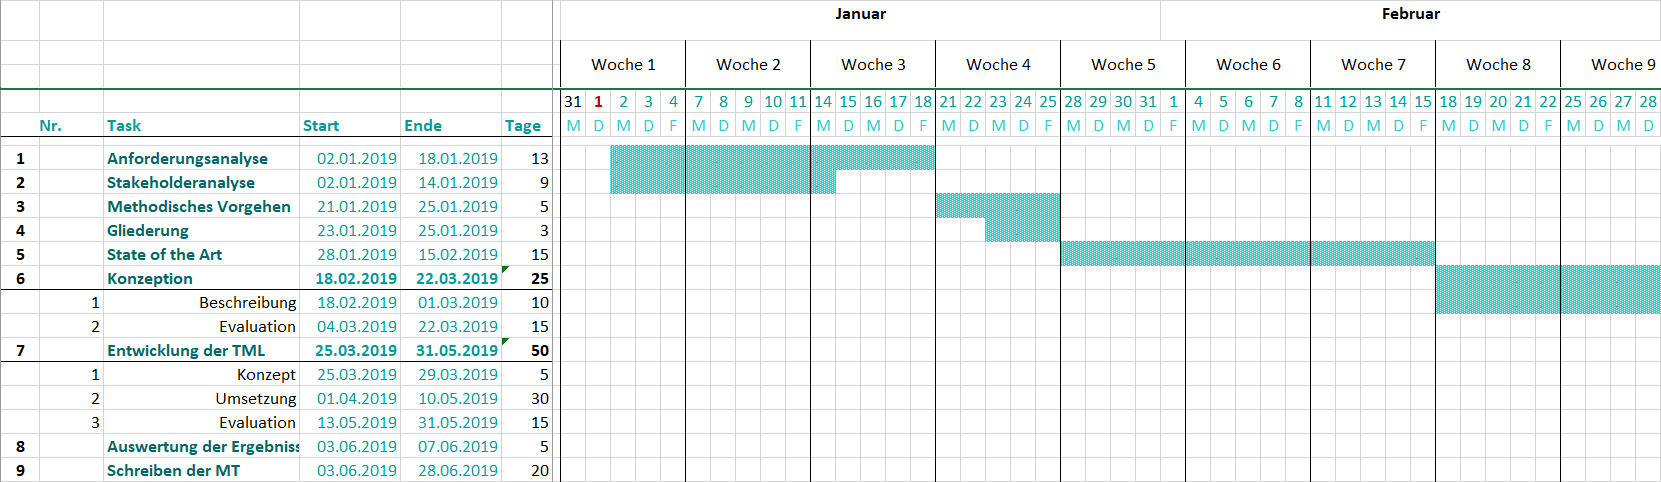
\includegraphics[scale=0.5, angle=90]{images/ganttG1.png}
%	\end{minipage}
%	\begin{minipage}{0.5\textwidth}
%		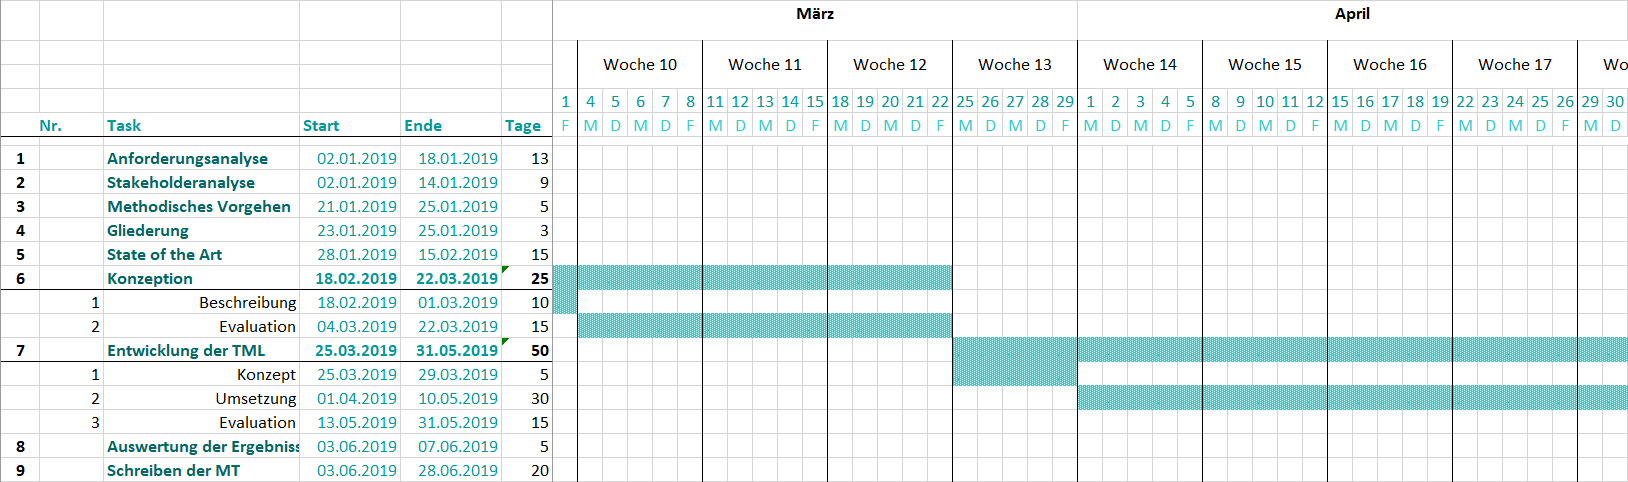
\includegraphics[scale=0.5, angle=90]{images/ganttG2.png}
%	\end{minipage}		
%\end{figure}
%
%\begin{figure}[h]	
%	\begin{minipage}{1\textwidth}
%		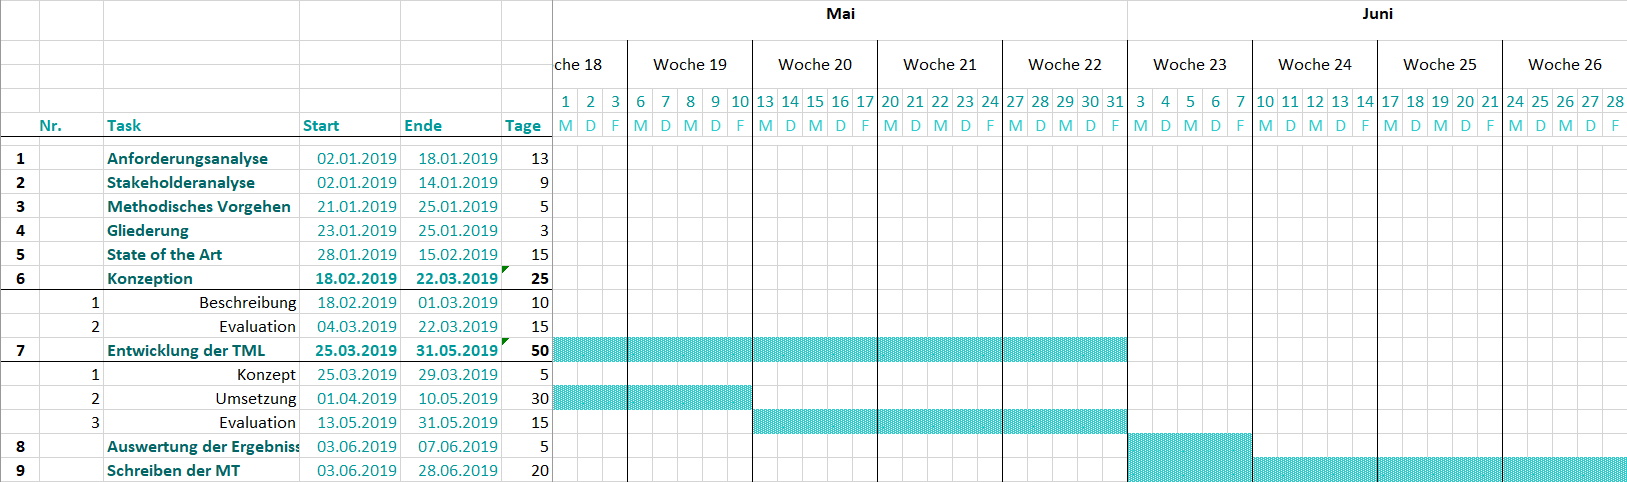
\includegraphics[scale=0.5, angle=90]{images/ganttG3.png}
%	\end{minipage}
%\end{figure}

\begin{figure}[h]
	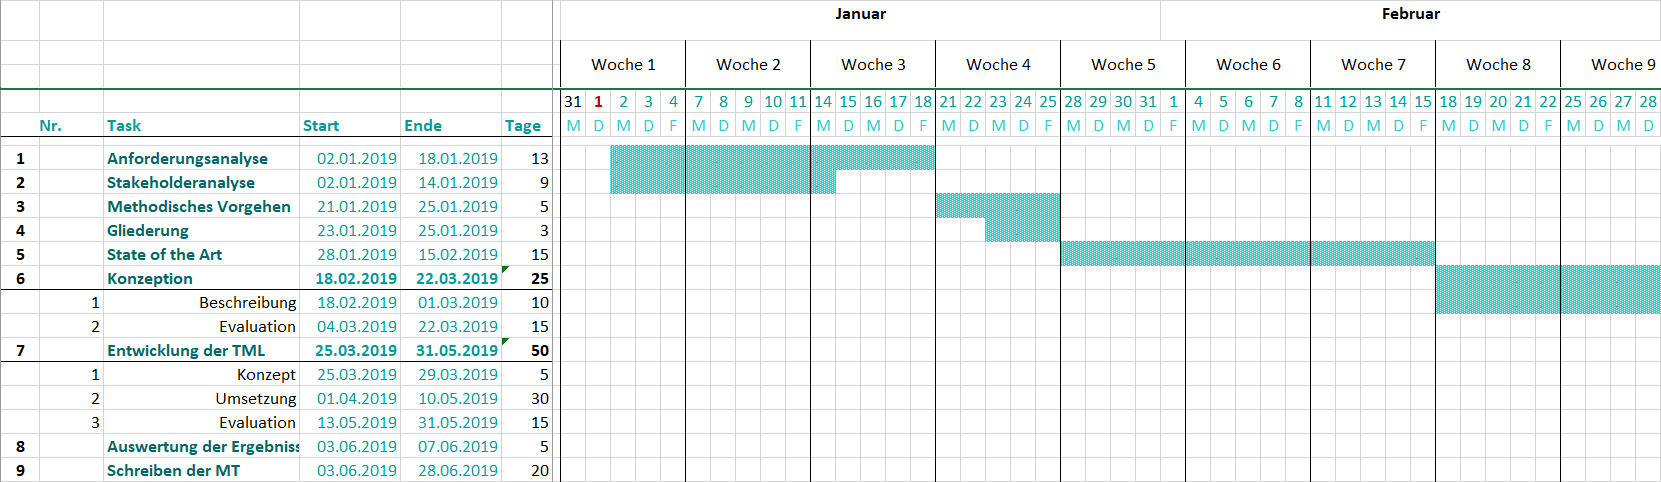
\includegraphics[scale=0.43]{images/ganttG1.png}
	\newline
	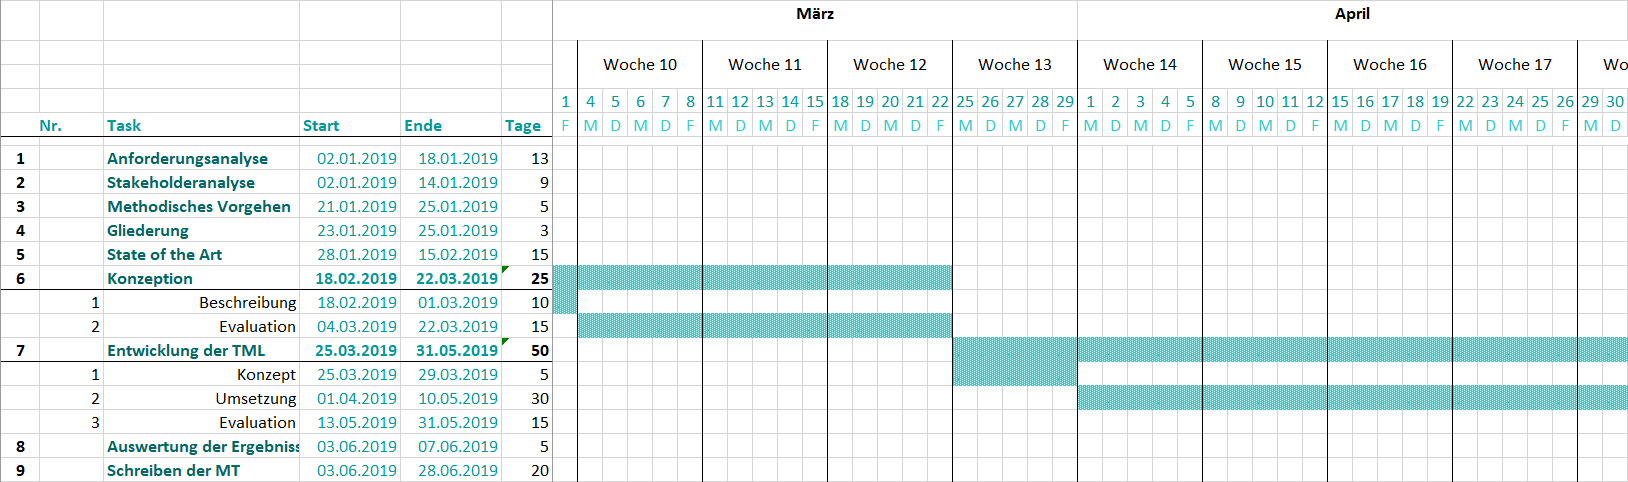
\includegraphics[scale=0.43]{images/ganttG2.png}
	\newline
	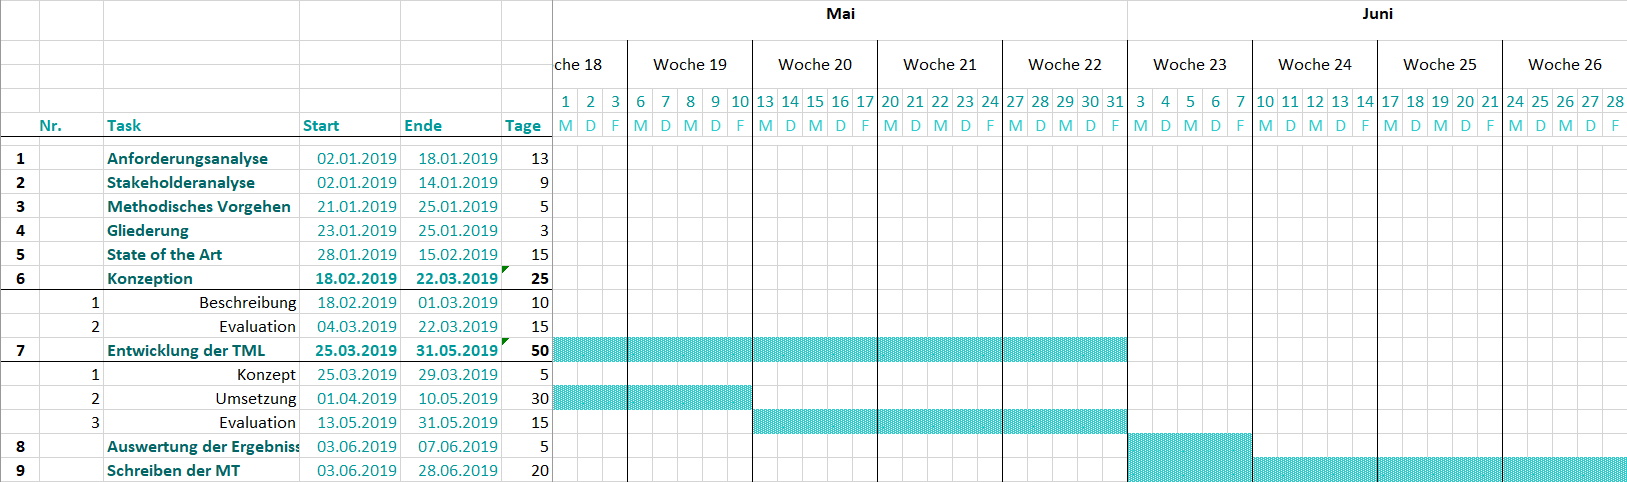
\includegraphics[scale=0.43]{images/ganttG3.png}	
\end{figure}





        % Evaluierung

%% ++++++++++++++++++++++++++++++++++++++++++
%% Anhang
%% ++++++++++++++++++++++++++++++++++++++++++

\appendix
%\include{anhang_a}
%\include{anhang_b}

%% ++++++++++++++++++++++++++++++++++++++++++
%% Literatur
%% ++++++++++++++++++++++++++++++++++++++++++
%  mit dem Befehl \nocite werden auch nicht 
%  zitierte Referenzen abgedruckt
\cleardoublepage
\phantomsection
\addcontentsline{toc}{chapter}{\bibname}
%%
%\nocite{*} % nur angeben, wenn auch nicht im Text zitierte Quellen 
           % erscheinen sollen
%\bibliographystyle{itmabbrv} % mit abgekürzten Vornamen der Autoren
%\bibliographystyle{gerplain} % abbrvnat unsrtnat
% spezielle Zitierstile: Labels mit vier Buchstaben und Jahreszahl
%\bibliographystyle{itmalpha}  % ausgeschriebene Vornamen der Autoren
\printbibliography
%% ++++++++++++++++++++++++++++++++++++++++++
%% Index
%% ++++++++++++++++++++++++++++++++++++++++++
\ifnotdraft{
\cleardoublepage
\phantomsection
\printindex            % Index, Stichwortverzeichnis
}
\end{document}
%% end of file

